% Generated from the public primitive catalog. Original Atlas drawing; Apache-2.0.
% Target: sha3-384; view: overview-compact
\documentclass[border=9pt]{standalone}
% Original Atlas figure theme. Apache-2.0; see the repository LICENSE.
\usepackage[T1]{fontenc}
\usepackage{lmodern}
\usepackage{amsmath,amssymb}
\usepackage{tikz}
\usetikzlibrary{arrows.meta,positioning,calc,fit,backgrounds,decorations.pathreplacing,matrix}
\definecolor{atlasInk}{HTML}{172235}
\definecolor{atlasTeal}{HTML}{0D7B7D}
\definecolor{atlasMuted}{HTML}{637278}
\definecolor{atlasFill}{HTML}{EAF4F2}
\definecolor{atlasLine}{HTML}{B6C8C7}
\tikzset{
  every picture/.style={line width=.65pt,draw=atlasInk,>=Latex},
  every node/.style={text=atlasInk,font=\sffamily\small},
  box/.style={draw,rounded corners=1.5pt,minimum height=.9cm,minimum width=1.6cm,align=center,inner sep=6pt,fill=white},
  accent/.style={box,draw=atlasTeal,fill=atlasFill},
  wire/.style={->,line width=.7pt},
  keywire/.style={wire,draw=atlasTeal,dashed},
  xor/.style={draw,circle,fill=white,inner sep=0pt,minimum size=.38cm},
  add/.style={draw,rectangle,fill=white,inner sep=0pt,minimum size=.38cm},
  note/.style={font=\sffamily\scriptsize,text=atlasMuted,align=center},
  phase/.style={font=\sffamily\small\bfseries,text=atlasTeal},
  group/.style={draw=atlasLine,dashed,rounded corners=2pt,inner sep=8pt}
}
\newcommand{\rotl}{\mathbin{\lll}}
\newcommand{\rotr}{\mathbin{\ggg}}
\newcommand{\kx}{\operatorname{Keccak}\!\text{-}\!f[1600]}

\newcommand{\AtlasKeyBits}{k}
\newcommand{\AtlasKeyWords}{N_k}
\newcommand{\AtlasRounds}{N_r}
\newcommand{\AtlasPriorRounds}{N_r-1}
\newcommand{\AtlasRoundKeys}{N_r+1}
\newcommand{\AtlasDoubleRounds}{N_r/2}
\newcommand{\AtlasSixRoundGroups}{N_r/6}
\newcommand{\AtlasFLGroups}{N_r/6-1}
\newcommand{\AtlasRoundStart}{24-n}
\newcommand{\AtlasBlockBits}{b}
\newcommand{\AtlasOutputBits}{384}
\newcommand{\AtlasStateBits}{1600}
\newcommand{\AtlasNonceBits}{v}
\newcommand{\AtlasCounterBits}{q}
\newcommand{\AtlasStreamBlockBits}{b}
\newcommand{\AtlasRate}{832}
\newcommand{\AtlasCapacity}{768}
\newcommand{\AtlasSteps}{N}
\newcommand{\AtlasLastStep}{N-1}
\newcommand{\AtlasWordBits}{200}
\newcommand{\AtlasHashWords}{50}
\newcommand{\AtlasFeedForward}{\boxplus}
\newcommand{\AtlasByteOrder}{big-endian}
\newcommand{\AtlasDomain}{01}
\newif\ifAtlasXof
\AtlasXoffalse
\begin{document}
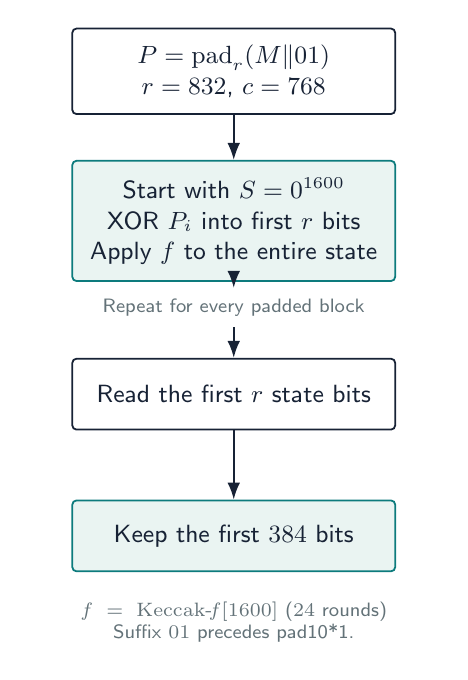
\begin{tikzpicture}
  \node[box,minimum width=4.1cm] (pad) at (0,0) {$P=\operatorname{pad}_r(M\Vert\AtlasDomain)$\\$r=\AtlasRate$, $c=\AtlasCapacity$};
  \node[accent,minimum width=4.1cm] (absorb) at (0,-1.9) {Start with $S=0^{1600}$\\XOR $P_i$ into first $r$ bits\\Apply $f$ to the entire state};
  \draw[wire] (pad) -- (absorb);
  \node[note] at (0,-3) {Repeat for every padded block};
  \node[box,minimum width=4.1cm] (read) at (0,-4.1) {Read the first $r$ state bits};
  \draw[wire] (absorb.south) -- (0,-2.75); \draw[wire] (0,-3.25) -- (read);
  \ifAtlasXof
    \node[accent,minimum width=4.1cm] (out) at (0,-5.9) {Need more output?\\Apply $f$, read $r$ bits again};
    \node[note] at (0,-7) {Return the requested $d$ bits};
    \node[note,text width=5cm] at (0,-7.8) {$f=\kx$ ($24$ rounds)\\Suffix $\AtlasDomain$ precedes pad10*1.};
  \else
    \node[accent,minimum width=4.1cm] (out) at (0,-5.9) {Keep the first $\AtlasOutputBits$ bits};
    \node[note,text width=5cm] at (0,-7) {$f=\kx$ ($24$ rounds)\\Suffix $\AtlasDomain$ precedes pad10*1.};
  \fi
  \draw[wire] (read) -- (out);
\end{tikzpicture}

\end{document}
